\chapter{Case study 2: Creating new constraints}
\label{chap:case_study2}

The \ref{chap:case_study1} chapter only showed the capabilities of the Konstrainer framework, but did not show how to write a more advanced script, because the \nameref{chap:konst_dsl} chapter was a prerequisite for that. This chapter will continue the case study.

\section{Writing your own policies}

Let's assume the company has introduced some custom policies and, now they want to enforce them using Konstrainer. Start with a very simple policy: All images must come from the internal company registry.

To enforce this, first let's detect which pods violate this policy:

Create a file with the company-policies.kt file with the following content:

\begin{lstlisting}[caption={Report skeleton},language=Kotlin,label=code:todo]
package me.btieger

import me.btieger.dsl.*

const val companyPrefix = "tiegris/"
val companPolicies = server("company-policies") {
  report {

  }
}
\end{lstlisting}

This script has an empty report so far. As described in the \ref{sec:report} section, we should fetch the list of pods and create an aggregation group. In this case, no additional processing is needed.

\begin{lstlisting}[caption={Aggregation group},language=Kotlin,label=code:todo]
report {
  val pods = kubelist { pods() }
  aggregation("Pods", pods) {

  }
}
\end{lstlisting}

To decide if all the containers of a pod are using images only from the company registry, we must specify this requirement with mathematical precision, using first order logic. Here are two continuous sentences which, express the requirement with first order logic.

`Tag the pod, if any of its containers image does not start with the company prefix.'

`Do not tag the pod, if all of its containers image starts with the company prefix.'

\begin{lstlisting}[caption={Tag pods},language=Kotlin,label=code:todo]
report {
  aggregation("Pods", kubelist { pods() }) {
    tag("Image not from company registry") {
      item.spec.containers.any { !it.image.startsWith(companyPrefix) }
    }
  }
}
\end{lstlisting}

The script accesses the Kubernetes API, but to do that successfully, it needs authorization. We need to associate a \emph{ClusterRole} to the agent. In the demo files there is also a \emph{ClusterRole} definition. We want our agent to be least privileged, so we are only giving it read access to the pods.

\begin{lstlisting}[caption={TODO},language=Kotlin,label=code:todo]
package me.btieger
import me.btieger.dsl.*

const val companyPrefix = "tiegris/"
val companyPolicies = server("company-policies") {
  clusterRole = "read-pods"
  report {
    aggregation("Pods", kubelist { pods() }) {
      tag("Image not from company registry") {
        item.spec.containers.any { !it.image.startsWith(companyPrefix) }
      }
    }
  }
}
\end{lstlisting}

The line: `clusterRole = ReadAny` assigns the ReadAny clusterrole to the agent by creating a clusterrolebinding during the deployment of the agent. The ReadAny clusterrole is created with the Konstrainer installation, it gives read access to all resources in the cluster.

Let's test the script now. If we upload, and deploy the script, we should see it working:

\begin{figure}[h]
  \centering
  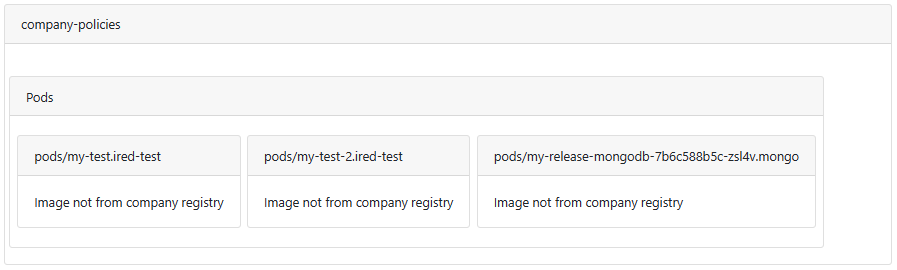
\includegraphics[width=130mm, keepaspectratio]{content/60_caseStudy2/company_policies_1.png}
  \caption{Report generated by the script}
  \label{fig:report}
\end{figure}

The report shows that there are 3 pods, which use images outside from the company registry.

Now lets do the enforcing part. Put this code inside the server block.

\begin{lstlisting}[caption={TODO},language=Kotlin,label=code:todo]
webhook("only-internal-registry") {
  operations(CREATE, UPDATE)
  apiGroups(APPS)
  apiVersions(ANY)
  resources(DEPLOYMENTS, STATEFULSETS, DAEMONSETS)
  namespaceSelector { }
  failurePolicy(FAIL)
  behavior {
    allowed {
      podSpec!!.containers.all { it.image.startsWith(companyPrefix) }
    }
    status {
      message = "All images must be from the company registry."
    }
  }
}
\end{lstlisting}

To create a rule, we need to add a `webhook` block. It needs a unique name. Lets name it "only-internal-registry". We need to define which events should the webhook listen to. In this example the webhook listens to the creation or update of any deployments, statefulsets and daemonsets.

The more interesting part is the behavior block. It describes how should the webhook behave when a request arrives. Inside the behavior block we can access the request body using many ways. One of them is the podSpec keyword. It is a shortcut to the `.spec.template.spec` of a deployment, statefulset or daemonset.

In the allowed block we can specify when to allow or reject an event. In this case we only accept events when the all the containers of the pod has an image starting with the the company prefix.

In the status block we define the error message in case the event is rejected.

Lets deploy and test our newly created agent dsl. On the monitors view we can see that the pods inside the ired-test namespace use images outside of the company registry, and the mongodb also uses an image from docker.io instead of the company registry.

We can also test that we can no longer create resources which use images outside from the company registry:

\begin{lstlisting}[caption={TODO},language=bash,label=code:bashx]
kubectl create ns policy-test
kubectl apply -f k8s/test-policy.yaml -n policy-test
\end{lstlisting}

We should get this error:

\begin{lstlisting}[caption={TODO},language=bash,label=code:todo]
Error from server: error when creating "k8s/test-policy.yaml": admission webhook "only-internal-registry.btieger.me" denied the request: All images must be from the company registry.
\end{lstlisting}

\begin{lstlisting}[caption={TODO},language=bash,label=code:bashx]
yq eval 'select(.kind == "Deployment").spec.template.spec.containers[0].image = "tiegris/apples-users"' k8s/test-policy.yaml -i
kubectl apply -f k8s/test-policy.yaml -n policy-test
\end{lstlisting}

This error shows that our rule works and is enforced.

This is the end of the demo. In this demo we saw the basic capabilities of the Konstrainer platform, some use-cases, and how to create our own rules.
